\documentclass[lettersize,journal]{IEEEtran}
\usepackage{amsmath,amsfonts}
\usepackage{algorithmic}
\usepackage{algorithm}
\usepackage{array}
\usepackage[caption=false,font=normalsize,labelfont=sf,textfont=sf]{subfig}
\usepackage{textcomp}
\usepackage{stfloats}
\usepackage{url}
\usepackage{verbatim}
\usepackage{graphicx}
\usepackage{cite}
\hyphenation{op-tical net-works semi-conduc-tor IEEE-Xplore}
% updated with editorial comments 8/9/2021

% \usepackage{amsmath,amsfonts}
% \usepackage{algorithmic}
% \usepackage{array}
% \usepackage[caption=false,font=normalsize,labelfont=sf,textfont=sf]{subfig}
% \usepackage{cite}
% \usepackage{textcomp}
% \usepackage{stfloats}
% \usepackage{url}
% \usepackage{verbatim}
% \usepackage{graphicx}
\usepackage{amssymb}
\usepackage{xcolor}
% \usepackage{appendix}
% \usepackage{algorithm}
\usepackage{amsthm}
% \usepackage{multirow} 
% \usepackage{multicol} 
% \usepackage{color}
\usepackage{bm}
% \hyphenation{op-tical net-works semi-conduc-tor IEEE-Xplore}
\usepackage{hyperref}
\usepackage{scalerel}
\usepackage{float}%提供float浮动环境
\usepackage{booktabs}%提供命令\toprule、\midrule、\bottomrule
\newtheoremstyle{custom}
  {\topsep}    % 上方间距
  {\topsep}    % 下方间距
  {\normalfont} % 定理内容的字体 (普通字体)
  {1em}           % 缩进量
  {\itshape}   % 定理标题的字体 (斜体)
  {:}          % 标题后的标点符号
  { }          % 标题后与内容的间距
  {\thmname{\textit{#1}}% 定理标题格式 (斜体)
   \thmnumber{ \textit{#2}}% 定理编号格式 (斜体)
   \thmnote{ \textit{(#3)}}}% 定理备注格式 (斜体)
% 应用自定义样式
\theoremstyle{custom}
\newtheorem{Thm}{Theorem}
\newtheorem{Lem}{Lemma}
\newtheorem{Cor}{Corollary}
\newtheorem{Def}{Definition}
\newtheorem{Exam}{Example}
\newtheorem{Alg}{Algorithm}
\newtheorem{Prob}{Problem}
\newtheorem{subproblem}{Problem}[Prob]
\newtheorem{Rem}{Remark}
\newcommand{\RNum}[1]{\uppercase\expandafter{\romannumeral #1\relax}}
\newcommand{\tabincell}[2]{\begin{tabular}{@{}#1@{}}#2\end{tabular}}
% \theoremseparator{:}
\newtheorem{hyp}{Hypothesis}

\begin{document}

\title{A TREE Oriented Embodied AI Multiplexing Framework for Green 6G Networks}

\author{IEEE Publication Technology,~\IEEEmembership{Staff,~IEEE,}
        % <-this % stops a space
\thanks{This paper was produced by the IEEE Publication Technology Group. They are in Piscataway, NJ.}% <-this % stops a space
\thanks{Manuscript received April 19, 2021; revised August 16, 2021.}}

% The paper headers
\markboth{Journal of \LaTeX\ Class Files,~Vol.~14, No.~8, August~2021}%
{Shell \MakeLowercase{\textit{et al.}}: A Sample Article Using IEEEtran.cls for IEEE Journals}

\IEEEpubid{0000--0000/00\$00.00~\copyright~2021 IEEE}
% Remember, if you use this you must call \IEEEpubidadjcol in the second
% column for its text to clear the IEEEpubid mark.

\maketitle

\begin{abstract}
This document describes the most common article elements and how to use the IEEEtran class with \LaTeX \ to produce files that are suitable for submission to the IEEE.  IEEEtran can produce conference, journal, and technical note (correspondence) papers with a suitable choice of class options. 
\end{abstract}

\begin{IEEEkeywords}
Article submission, IEEE, IEEEtran, journal, \LaTeX, paper, template, typesetting.
\end{IEEEkeywords}

\section{Introduction}
\IEEEPARstart{X}{xx}...  
Multi-modal sensor fusion and unstructured environment are identified as two key features of embodied AI \cite{li_developments_2025}. However, xxx. 
Wireless communication is also identified as a crucial enabling technology for embodied robotics, especially humanoid and xxx, for the flexible and ubiquitous characteristics. 

In order to fuse the multi-modal sensory data and adapt into the dynamic unstructured environments, xxx AI-assisted methods have been proposed. In the early researches, xxx. Due to its multi-task emergence abilities, VLA has become a heated research topic. \cite{}, \cite{}, \cite{} performs high-accuracy action inference in a xxx of embodied tasks. However, these architectures overlook xxx, xxx in practical deployments. 

For practical deployment, several architectures are developed to mitigate the xxx. The embodied LAM architectures are mainly divided into 2 architectures, end-to-end VLA and dual system. End-to-end VLA includes xxx, xxx, and xxx. They xxx. However the end-to-end architectures xxx and suffer latency and power consumption draw-backs on humanoid and xxx embodied systems. To mitigate these drawbacks, dual system, including Helix, InternVLA, GR00T, xxx. Although the dual system embodied AI architectures xxx, they still fail to adapt into dynamic and resource limited wireless systems. 

To fill this gap, recent token pruning methods \cite{}, \cite{} manage to reduce token overhead. xxx. WNCS techniques \cite{}, \cite{}, \cite{} are also one of the candidate techniques to xxx. Semantic-aware and goal-oriented methods \cite{}, \cite{}, \cite{} xxx. Despite the corresponding performance improvements spotted in the up-mentioned methods, the fundamental performance bound for hybrid VLA data transmission under wireless links is still uninvestigated. 

Motivated by these, our main contributions are summarized as follows: 
\begin{itemize}
    \item \bf{xxx} xxx. 
    \item \bf{xxx} xxx. 
    \item \bf{xxx} xxx. 
\end{itemize}

And the rest of the paper are organized as follows. xxx. 

\section{System Model}
In this paper, we study a wireless-enabled embodied AI (WEEA) system, where an embodied agent and the corresponding sensing nodes $\mathcal{S} = \{1, \ldots, s, \ldots, S\}$ are connected to the edge remote controller $e$ with Vision-Language-Action (VLA) equipped. 
% $I$ agents with sensing and action abilities are distributed in the space. 
The system is illustrated in Fig.~\ref{}. Each sensing node perceives the environment with observations $\mathcal{V}_s(t) \in \mathcal{V}(t)$ (e.g., RGB images), its raw data volume is identified with $d_s(t)$. The edge VLA model receive $\mathcal{V}(t)$ and a time-invariant language instruction (prompt) $p$, then predict an action sequence $\mathcal{A}(t)$ (e.g., end-effector poses or joint velocities), $\Pi_\theta(\mathcal{A}(t) \vert \mathcal{V}(t), p)$, where $\theta$ denotes the VLA model parameter. 
% singel-cell system where the base station (BS) is equipped with edge computing power, serving a set of user equipments (UEs), denoted by $i \in \mathcal{I}$. 
% Each agent contains hybrid content transmissions of multi-modal sensory data from helper agent $j$ to ego agent $i$, denoted with ${\bf d}_{j, i}(t) = \{ d^\mathrm{v}_{j, i}(t), d^\mathrm{r}_{j, i}(t), \ldots \}$, where $d^\mathrm{v}_{j, i}(t)$, $d^\mathrm{r}_{j, i}(t)$ represent the transmission data volume of vision, radar, etc., from helper agent $j$ to ego agent $i$, respectively. 
% Each agent contains hybrid content transmissions of multi-modal sensory data and control data, profiled with ${\bf q}_i(t) = \{ {\bf q}^\mathrm{v}_i(t), {\bf q}^\mathrm{r}_i(t), {\bf q}^\mathrm{ms}_i(t), \ldots , {\bf q}^\mathrm{mc}_i(t) \}$, where ${\bf q}^\mathrm{v}_i(t) = \{ {\bf d}^\mathrm{v}_i(t), f^\mathrm{v} \}$, ${\bf q}^\mathrm{r}_i(t) = \{ {\bf d}^\mathrm{r}_i(t), f^\mathrm{r} \}$, ${\bf q}^\mathrm{ms}_i(t) = \{ d^\mathrm{ms}_i(t), f^\mathrm{ms} \}$ and ${\bf q}^\mathrm{mc}_i(t) = \{ d^\mathrm{mc}_i(t), f^\mathrm{mc} \}$ represent the transmission profile of vision, radar, motor state and motor control for agent $i$, including data volume and transmission frequency, respectively. 


% \subsection{xxx Protocol Design}
% Identifying the multi-modal sensory feedback

% The communication resource grid is 



% Puncturing\footnote{xxx} and finite block-length short packet transmission are enabled for ultra low-latency high-reliability motor state and control signal transmissions. The puncturing duration at sub-channel $f$ is denoted by $t_{i, f} < T_k, i \in \mathcal{I}_{m}$. 
% % Puncturing\footnote{xxx} is enabled for ultra low-latency high-reliability transmissions, which is suitable for text queries transmissions carrying more semantic information within each bits \cite{}. 

\subsection{Communication Model}
The up-link transmission rate from sensing node $s$ to the edge server at slot $t$ is described as
\begin{align}
    r_{s}(t) = B_s(t) \log_2\left(1 + \mathrm{SNR}_s(t) \right), \forall s \in \mathcal{S}, 
\end{align}
where $B_s(t)$ and $\mathrm{SNR}_s(t)$ denote the bandwidth allocated to $s$ and the signal-to-noise ratio (SNR) of $s$, respectively. Let $\tau$ denote the duration of one sensing--communication--control slot. The bandwidth allocation follows
\begin{align}\label{bandwidth_cons}
    \sum_{s \in \mathcal{S}}B_s(t) \leq B, 
\end{align}
where $B$ is the system bandwidth\footnote{We assume that adequate bandwidth $B$ is semi-persistently allocated to the WEEA system via orthogonal radio access network (RAN) slicing techniques \cite{}, \cite{}}. 

% The transmission rate from helper agent $j$ to ego agent $i$ at slot $t$ is described as: 
% \begin{align}
%     r_{j, i}(t, f) = B \sum_{f \in \mathcal{F}} b_{f, j, i}(t) \log_2\left(1 + \frac{p_{j, i}(t) h_{j, i}(t)}{\vartheta^2} \right), 
%     % i \in \mathcal{I}_i \cup \mathcal{I}_v &, 
% \end{align}
% % \begin{align}
% %     r_{n, i}(t, f) = (1 - \sum_{i \in \mathcal{I}_\mathrm{t}}\frac{t_{i, f}}{T_k})\log_2\left(1 + \frac{p_{n, i}(t) h_{n, i}(t)}{\vartheta^2} \right) &, \nonumber\\
% %     i \in \mathcal{I}_i \cup \mathcal{I}_v &, 
% % \end{align}
% where $h_{j, i}(t)$ is the channel coefficient from $j$ to $i$, $B$ is unit bandwidth of sub-channel, $\vartheta$ is the xxx and $b_{f, j, i}(t)$, $p_{j, i}(t)$ is the sub-channel allocation indicator and the transmit power, respectively. $b_{f, j, i}(t) = 1$ means sub-channel $f$ is allocated for the data transmission from $j$ to $i$ and $b_{f, j, i}(t) = 0$ otherwise.  The transmit power of each agent $i$ is bounded by 
% \begin{align}
%     \sum_{i \in \mathcal{I}, i \neq j} p_{j, i}(t) \leq P_\mathrm{max}. 
% \end{align}
% Transmission power consumption \cite{xu_energy-efficient_2013} for each BS $n$ is given as
% \begin{align}
%     P_{n}^{\mathrm{com}} = P_S + \alpha \cdot P_T
% \end{align}
% where $P_S$ and $\alpha$ represents the static circuit power and the power amplification coefficient, respectively. 

\subsection{Top-$k$-enabled Token Compression Model}
% Each edge server cache a set of $\mathcal{L}_n$ LAMs. 
In order to support timely and efficient perceptional data delivery, top-$k$ Token compression techniques are widely investigated \cite{}, \cite{}. 

Through tokenization and top-$k$ token pruning, the raw observation $\mathcal{V}_s(t)$ is locally converted into $n_s$ visual tokens and only $k_s(t)$ tokens are retained for uplink transmission. The corresponding air-interface data volume is modeled as
\begin{align}
    d_s^{k_s}(t) = \frac{\alpha_s k_s(t)}{n_s} d_s(t), \quad \forall s \in \mathcal{S},
    \label{token_volume}
\end{align}
where $\alpha_s$ captures the tokenizer-dependent feature-bit expansion/compression factor, $n_s$ is the original visual-token length, and $k_s(t)\in\{k_s^{\min},\ldots,n_s\}$ is the retained token length at slot $t$. We define the slot-wise pruning decision vector as ${\bf k}(t)=\{k_1(t),\ldots,k_S(t)\}$.

With top-$k$ token compression, the edge VLA receives an incomplete multi-view observation and may therefore suffer action degradation. We characterize the long-term action distortion by
\begin{align}
    \epsilon_{\bf k}
    = \frac{1}{T}\mathbb{E}\left[
    \sum_{t=1}^{T}
    \left\|\mathcal{A}_{{\bf k}(t)}(\mathcal{V}(t))
    -\mathcal{A}^{*}(\mathcal{V}(t))\right\|_2^2
    \right],
    \label{action_mse}
\end{align}
where $\mathcal{A}_{{\bf k}(t)}(\mathcal{V}(t))$ denotes the action generated from the pruned multi-view tokens and $\mathcal{A}^{*}(\mathcal{V}(t))$ denotes the reference action obtained from the unpruned observations. 

% The transmission data volume from helper agent $j$ to ego agent $i$ with top-$k$ Token pruning \cite{} is given by 
% \begin{align}
%     d^\mathrm{v}_{j, i}(t) = \frac{k^\mathrm{v}_{j, i}}{n^\mathrm{v}}D^\mathrm{v}_{j, i}(t), 
% \end{align}
% % where xxx. And the corresponding QoS metrics for each LAM in terms of accuracy and delay are listed as follows
% where ${\bf k} = \{ \{k^\mathrm{v}_{j, i}\}, \{k^\mathrm{r}_{j, i}\}, \ldots \}$ denotes the whole set of top-$k$ Token pruning rate. 

% And the corresponding VLA inference action error requirement of agent $i$ is listed as follows
% \begin{align}\label{accuracy_cons}
%     \epsilon_i({\bf k}, t) \leq \delta_i, \forall i \in \mathcal{I}, 
% \end{align}
% % \begin{align}\label{accuracy_delay_cons}
% % \left\{
% %     \begin{array}{l l}
% %         q() \geq \rho_l, \forall l \in \mathcal{L}_n, \forall n \in \mathcal{N}_{BS}, \\
% %         d() \leq \delta_l, \forall l \in \mathcal{L}_n, \forall n \in \mathcal{N}_{BS}. 
% %     \end{array}
% % \right. 
% % \end{align}
% where $\epsilon_i({\bf k})$ and $\delta_i$ denotes the VLA inference error and error threshold of agent $i$, respectively. 
% % where $\rho_l$ and $\delta_l$ are corresponding accuracy and delay thresholds of LAM $l$. 

% Computing power consumption for each agent $i$ is given according to the well investigated dynamic voltage and frequency scaling (DVFS) \cite{guerreiro_modeling_2019} as follows
% \begin{align}
%     P_{i}^{\mathrm{comp}} = 
% \end{align}

\section{Problem Formulation}
We first formulate the original action-error minimization problem as follows.
\begin{Prob}[Original Action Error Minimization Problem]
    The action error of the WEEA system is minimized by jointly optimizing the per-view token-retention lengths and uplink bandwidth allocation:
    \begin{align}
        \underset{\{{\bf k}(t),B_s(t)\}_{t=1}^{T}}{\textrm{minimize}} \quad & \epsilon_{\bf k} \nonumber\\
        \textrm{subject to} \quad
        & \tau r_s(t) \geq d_s^{k_s}(t), \quad \forall s,t, \label{rate_cons}\\
        & k_s^{\min} \leq k_s(t) \leq n_s, \quad k_s(t)\in\mathbb{Z}, \quad \forall s,t, \label{k_cons}\\
        & \eqref{bandwidth_cons}. \nonumber
    \end{align}
\end{Prob}

Problem 1 is difficult to solve directly for three reasons. First, the mapping from the multi-view pruning vector ${\bf k}(t)$ to the downstream VLA action error in \eqref{action_mse} is a high-dimensional black-box function without an explicit analytical form. Second, the task relevance of each view is time varying because the action-generation process attends to different spatial regions and camera views at different manipulation stages. Third, the action-related internal signal is only available after edge-side VLA inference; hence, the feedback obtained at the end of slot $t-1$ can only be used for the pruning decision at slot $t$. This one-slot causal delay prevents the direct use of the instantaneous action relevance for token allocation.

To address these challenges, we construct an action-relevance surrogate from the internal cross-attention of the edge VLA, compensate for its one-slot feedback delay by temporal prediction, and transform Problem 1 into a weighted concave token-allocation problem with an analytical water-filling structure. 
% To start with, we have the cost-efficiency ratio of the WEEA system denoted as: 
% \begin{align}
%     \eta = 
% \end{align}
% % To start with, we have the cost-efficiency ratio of the embodied LAM system denoted as
% % \begin{align}
% %     \eta_{xxx} = \frac{\sum_{i} \alpha_i({\bf k}, t)}{\sum_j \sum_{i \in \mathcal{I}, i \neq j} p_{j, i}(t) + \sum_{i} P^{comp}_i}, 
% % \end{align}
% % where $\alpha_i({\bf k}, t)$ stands for the xxx. 
% % To start with, we have the token responsive energy-efficiency metric \cite{yu_tree_2026} for the distributed MLAM inference-integrated edge BS system denoted as 
% % \begin{align}
% %     \eta_{TREE} = \frac{\displaystyle\sum_{n \in \mathcal{N}_{BS}}\displaystyle\sum_{l \in \mathcal{L}_n}\beta_l \cdot T_l}{\displaystyle\sum_{n \in \mathcal{N}_{BS}}(P_{n}^{\mathrm{com}} + P_{n}^{\mathrm{comp}})}
% % \end{align}
% % where $\beta_l$ is the normalization factor converting tokens to bit-equivalent utility for cached LAM $l$\footnote{The normalization factor is determined corresponding to the token pricing strategies. For example, xxx, xxx, xxx. \cite{} }. 

% And the original cost-efficiency ratio optimization problem is given by 
% \begin{Prob}[Original Cost-efficiency Ratio Maximization Problem]
%     The cost-efficiency ratio of the xxx system can be maximized via the following optimization problem. 
%     \begin{align}
%         \underset{{\bf k}, \{B_s(t)\}}{\textrm{maximize}} && \eta \nonumber\\
%         \textrm{subject to} && r_s(t) \geq d_s^{k_s}(t), \forall s \in \mathcal{S}, \label{rate_cons}\\
%         && \eqref{bandwidth_cons}
%         % P_i^\mathrm{comp} \leq P_\mathrm{max}^\mathrm{comp}, \forall i \in \mathcal{I}, \label{computational_cons}\\
%         % && P_n^\mathrm{com} \leq P_\mathrm{max}^\mathrm{com}, \forall n \in \mathcal{N}_{BS}, \label{communication_cons}\\
%         % && \eqref{accuracy_cons}, \nonumber
%     \end{align}
% \end{Prob}
\section{Problem Transformation}
In this section, in order to investigate the high-dimensional black-box VLA action error characteristics, we carry out an analytical study with well-known GR00T N1.5 VLA model \cite{nvidia_gr00t_2025} and derive a xxx-based action-conditioned relevance score. Noting the posterior delay issue of the relevance score, a delay compensated relevance prediction framework is proposed. 

\subsection{Action-Conditioned View Relevance}
We exploit the internal action-generation signal of the edge VLA to quantify the marginal contribution of different camera views. This construction is particularly compatible with dual-system VLAs such as GR00T N1.5, in which vision-language embeddings are cross-attended by a diffusion-transformer (DiT) action model \cite{nvidia_gr00t_2025}. Let $\mathcal{J}_s(t)$ denote the indices of the visual tokens received from sensing node $s$ at slot $t$. For action-query index $q$, layer $l$, and attention head $h$, let $a_{q,s,j}^{l,h}(t)$ be the cross-attention weight assigned to token $j\in\mathcal{J}_s(t)$, and let ${\bf v}_{s,j}^{l,h}(t)$ denote the corresponding value vector. We define the action-conditioned relevance of token $j$ as
\begin{align}
    z_{s,j}(t)
    = \frac{1}{|\mathcal{L}||\mathcal{H}||\mathcal{Q}|}
    \sum_{l\in\mathcal{L}}\sum_{h\in\mathcal{H}}\sum_{q\in\mathcal{Q}}
    a_{q,s,j}^{l,h}(t)\left\|{\bf v}_{s,j}^{l,h}(t)\right\|_2,
    \label{token_relevance}
\end{align}
where $\mathcal{L}$, $\mathcal{H}$, and $\mathcal{Q}$ are the selected action-model layers, heads, and action queries, respectively. Compared with attention weight alone, \eqref{token_relevance} additionally accounts for the magnitude of the value vector and therefore better reflects the effective contribution entering the action representation. Action-conditioned attention has also been shown to be informative for VLA-specific visual-token pruning \cite{liu_vlapruner_2025}.

By carrying out numerical xxx ??? As illustrated in Fig.~\ref{}, we have the 
\begin{align}
    \frac{\partial \epsilon_{\bf k}}{\partial k_s} \propto \frac{p_s}{k_s + \kappa}, 
\end{align}

The view-level relevance is obtained by aggregating the retained tokens,
\begin{align}
    u_s(t) = \sum_{j\in\mathcal{J}_s(t)} z_{s,j}(t), \qquad
    p_s(t) = \frac{u_s(t)+\varepsilon}{\sum_{i\in\mathcal{S}}(u_i(t)+\varepsilon)},
    \label{view_relevance}
\end{align}
where $p_s(t)$ is the normalized action relevance and $\varepsilon>0$ avoids numerical singularity. The vector ${\bf p}(t)=[p_1(t),\ldots,p_S(t)]$ is fed back by the edge after inference and becomes available to sensing nodes before slot $t+1$.

\subsection{Delay-Compensated Relevance Prediction}
Because ${\bf p}(t)$ is generated only after the action at slot $t$ has been inferred, the current pruning decision cannot depend on ${\bf p}(t)$. We therefore use a causal one-step predictor. For $t\geq 3$, the predicted relevance is
\begin{align}
    \widetilde p_s(t)
    = \left[p_s(t-1)+\rho\big(p_s(t-1)-p_s(t-2)\big)\right]^+,
    \label{relevance_predictor}
\end{align}
where $\rho\in[0,1]$ controls the extrapolation strength and $[x]^+=\max(x,0)$. To prevent an abrupt manipulation-stage transition from causing over-confident allocation, we measure the temporal variation by
\begin{align}
    \Delta(t)=\frac{1}{2}\left\|{\bf p}(t-1)-{\bf p}(t-2)\right\|_1,
    \label{transition_metric}
\end{align}
and define an adaptive exploration factor
\begin{align}
    \eta(t)=\min\left\{\eta_{\max},\eta_0+\gamma\Delta(t)\right\}.
    \label{exploration_factor}
\end{align}
The robust predicted relevance used for allocation is then
\begin{align}
    \widehat p_s(t)
    = (1-\eta(t))
    \frac{\widetilde p_s(t)}{\sum_i\widetilde p_i(t)+\varepsilon}
    +\frac{\eta(t)}{S}.
    \label{robust_relevance}
\end{align}
When the action-relevance distribution evolves smoothly, $\eta(t)$ is small and the algorithm exploits the predicted task relevance. When a sudden relevance shift is detected, \eqref{robust_relevance} approaches a uniform distribution, preserving multi-view coverage until a reliable action-conditioned feedback signal is obtained.

\subsection{Bandwidth-Cost Transformation}
Combining \eqref{rate_cons}, \eqref{token_volume}, and the communication rate model yields the minimum bandwidth required to transmit $k_s(t)$ tokens within one slot:
\begin{align}
    B_s(t) \geq c_s(t)k_s(t),
    \label{bandwidth_per_token}
\end{align}
where
\begin{align}
    c_s(t)
    = \frac{\alpha_s d_s(t)}
    {n_s\tau\log_2(1+\mathrm{SNR}_s(t))}
    \label{token_bandwidth_cost}
\end{align}
is the effective bandwidth cost of retaining one visual token at sensing node $s$. Hence, the original communication constraints can be equivalently represented by
\begin{align}
    \sum_{s\in\mathcal{S}}c_s(t)k_s(t) \leq B.
    \label{weighted_token_budget}
\end{align}
This transformation explicitly couples task relevance and wireless conditions: a view receives more tokens when it is action critical, whereas a poor wireless link increases its per-token resource cost.

Since the exact action-MSE function is unavailable online, we use the predicted action relevance as a local surrogate of the marginal information value. To capture the diminishing return caused by redundant visual tokens, the retained-token utility of view $s$ is modeled by the concave function $\widehat p_s(t)\log(k_s(t)+\kappa)$, where $\kappa>0$. At each slot, Problem 1 is transformed into
\begin{Prob}[Action-Relevance-Aware Token Allocation]
\begin{align}
    \underset{\{k_s(t)\}}{\textrm{maximize}} \quad
    & \sum_{s\in\mathcal{S}}\widehat p_s(t)
    \log\big(k_s(t)+\kappa\big) \label{surrogate_obj}\\
    \textrm{subject to} \quad
    & \sum_{s\in\mathcal{S}}c_s(t)k_s(t)\leq B, \nonumber\\
    & k_s^{\min}\leq k_s(t)\leq n_s, \quad \forall s. \nonumber
\end{align}
\label{prob_surrogate}
\end{Prob}
The integer restriction is temporarily relaxed in Problem 2 and restored by a budget-feasible rounding step after optimization. We assume that the minimum multi-view coverage is feasible, i.e., $\sum_s c_s(t)k_s^{\min}\leq B$; otherwise, the system enters an outage state and the minimum-retention requirement must be relaxed.

\section{Proposed Solutions}
\subsection{Action-Relevance-Aware Weighted Water Filling}
Problem 2 is a concave maximization problem over a convex feasible set. Its continuous optimum therefore follows directly from the Karush--Kuhn--Tucker (KKT) conditions.

\begin{Thm}[Optimal token allocation]
For fixed $\widehat p_s(t)>0$ and $c_s(t)>0$, the optimal continuous token allocation of Problem 2 is
\begin{align}
    k_s^{\star}(t)
    = \left[
    \frac{\widehat p_s(t)}{\lambda^{\star}(t)c_s(t)}-\kappa
    \right]_{k_s^{\min}}^{n_s},
    \label{water_filling}
\end{align}
where $[x]_a^b=\min\{b,\max\{a,x\}\}$ and $\lambda^{\star}(t)\geq0$ is selected such that $\sum_s c_s(t)k_s^{\star}(t)=B$ whenever the bandwidth constraint is active.
\end{Thm}
\begin{proof}
The objective in \eqref{surrogate_obj} is strictly concave in $k_s(t)$ for every $\widehat p_s(t)>0$, while all constraints are affine. Ignoring the box constraints first, stationarity of the Lagrangian gives
$\widehat p_s(t)/(k_s(t)+\kappa)-\lambda(t)c_s(t)=0$.
Solving for $k_s(t)$ and applying complementary slackness for the lower and upper bounds yields \eqref{water_filling}. Since the weighted sum $\sum_s c_s(t)k_s^{\star}(t)$ is monotonically non-increasing in $\lambda(t)$, the unique multiplier can be obtained by bisection whenever the resource constraint is active.
\end{proof}

Equation \eqref{water_filling} reveals an intuitive importance-to-cost structure. The retained token length increases with the predicted action relevance $\widehat p_s(t)$ and decreases with the wireless token cost $c_s(t)$. After obtaining the continuous solution, we first set $k_s(t)=\lfloor k_s^{\star}(t)\rfloor$. Any residual bandwidth is greedily assigned one token at a time to the feasible sensing node with the largest instantaneous marginal utility per bandwidth,
\begin{align}
    g_s(t)=\frac{\widehat p_s(t)}{c_s(t)\big(k_s(t)+\kappa\big)},
    \label{rounding_gain}
\end{align}
until no additional token can be accommodated.

The minimum bandwidth allocation is subsequently set as
\begin{align}
    B_s^{\star}(t)=c_s(t)k_s(t),
    \label{optimal_bandwidth}
\end{align}
while unused bandwidth, if any, can be released to other network slices.

\subsection{Local Intra-View Token Pruning}
The edge feedback determines how many tokens each view should transmit, while the sensing node determines which tokens are retained. This separation keeps the sensing side lightweight and avoids running the action model locally. Let ${\bf x}_{s,j}(t)$ denote current visual token $j$ and $\bar{\bf x}_s(t)=n_s^{-1}\sum_j{\bf x}_{s,j}(t)$ denote the mean token feature. We use the following training-free local distinctiveness score:
\begin{align}
    q_{s,j}^{\mathrm{loc}}(t)
    = \left\|{\bf x}_{s,j}(t)-\bar{\bf x}_s(t)\right\|_2,
    \label{local_score}
\end{align}
where a larger value indicates that the token carries visual content less represented by the average view feature. Each sensing node transmits the $k_s(t)$ tokens with the largest $q_{s,j}^{\mathrm{loc}}(t)$. Importantly, the proposed inter-view allocation is agnostic to the specific intra-view selector; therefore, \eqref{local_score} can be replaced by an existing training-free saliency or redundancy-based token-pruning rule without modifying the action-relevance feedback and wireless resource allocation modules.

\begin{algorithm}[t]
\caption{Delayed Action-Relevance-Guided Token Allocation and Pruning}
\label{alg:darp}
\begin{algorithmic}[1]
\REQUIRE $B$, $\tau$, $\{n_s,k_s^{\min},\alpha_s\}_{s=1}^{S}$, predictor parameters $\rho,\eta_0,\eta_{\max},\gamma$, $\kappa$.
\ENSURE Slot-wise token allocation ${\bf k}(t)$ and bandwidth allocation ${\bf B}(t)$.
\STATE Initialize $p_s(0)=p_s(1)=1/S$, $\forall s$.
\FOR{$t=1,2,\ldots,T$}
    \STATE The edge/resource controller obtains the current uplink $\mathrm{SNR}_s(t)$ and computes $c_s(t)$ according to \eqref{token_bandwidth_cost}.
    \IF{$t\leq 2$}
        \STATE Set $\widehat p_s(t)=1/S$, $\forall s$.
    \ELSE
        \STATE Predict $\widetilde p_s(t)$ using \eqref{relevance_predictor}; compute $\Delta(t)$ and $\eta(t)$ using \eqref{transition_metric}--\eqref{exploration_factor}.
        \STATE Construct robust relevance $\widehat p_s(t)$ using \eqref{robust_relevance}.
    \ENDIF
    \STATE Find $\lambda^{\star}(t)$ by bisection and obtain $k_s^{\star}(t)$ from \eqref{water_filling}.
    \STATE Apply floor-and-greedy rounding using \eqref{rounding_gain}; set $B_s(t)=c_s(t)k_s(t)$ and signal $k_s(t)$ to sensing node $s$.
    \STATE At sensing node $s$, tokenize the current observation, compute \eqref{local_score}, retain the top-$k_s(t)$ tokens, and transmit them to the edge.
    \STATE Edge VLA performs action inference and computes token/view relevance using \eqref{token_relevance}--\eqref{view_relevance}.
    \STATE Store/feedback ${\bf p}(t)$, which becomes usable for the allocation of slot $t+1$.
\ENDFOR
\end{algorithmic}
\end{algorithm}

\section{Performance Analysis}
We next characterize the effect of delayed relevance feedback and the computational complexity of Algorithm~\ref{alg:darp}.

\begin{Lem}[One-slot prediction error]
Assume the normalized relevance sequence has bounded second-order temporal variation, i.e.,
\begin{align}
    |p_s(t)-2p_s(t-1)+p_s(t-2)|\leq \xi_s, \quad \forall s,t.
    \label{smooth_assumption}
\end{align}
For the full linear extrapolation case $\rho=1$, the predictor in \eqref{relevance_predictor} before non-negative projection satisfies
\begin{align}
    |p_s(t)-\widetilde p_s(t)|\leq\xi_s.
    \label{prediction_bound}
\end{align}
\end{Lem}
\begin{proof}
For $\rho=1$, the unprojected prediction is $2p_s(t-1)-p_s(t-2)$. Hence the prediction error is exactly the second-order difference $p_s(t)-2p_s(t-1)+p_s(t-2)$, whose magnitude is bounded by \eqref{smooth_assumption}. The projection $[\cdot]^+$ cannot increase the distance to the non-negative target $p_s(t)$.
\end{proof}
Lemma 1 shows that one-slot feedback does not necessarily cause an unbounded mismatch: under the temporal continuity typically observed in manipulation, the error is controlled by the curvature of the relevance trajectory rather than by its absolute value. The adaptive uniform component in \eqref{robust_relevance} further reduces the risk of view starvation when this temporal-smoothness assumption is temporarily violated.

\begin{Thm}[Surrogate-utility loss under relevance error]
Let ${\bf p}(t)$ be the ideal instantaneous normalized relevance and $\widehat{\bf p}(t)$ the causal estimate used by Algorithm~\ref{alg:darp}. Suppose $\|{\bf p}(t)-\widehat{\bf p}(t)\|_1\leq\delta_t$. Let ${\bf k}^{\mathrm{I}}(t)$ maximize Problem 2 using ${\bf p}(t)$ and ${\bf k}^{\mathrm{D}}(t)$ maximize it using $\widehat{\bf p}(t)$. Then
\begin{align}
    &\sum_s p_s(t)\log(k_s^{\mathrm{I}}(t)+\kappa)
    -\sum_s p_s(t)\log(k_s^{\mathrm{D}}(t)+\kappa) \nonumber\\
    &\qquad\leq 2\delta_t L_{\max},
    \label{utility_gap}
\end{align}
where $L_{\max}=\max_s\log(n_s+\kappa)$.
\end{Thm}
\begin{proof}
For any feasible ${\bf k}$,
$|\sum_s(p_s-\widehat p_s)\log(k_s+\kappa)|\leq\delta_t L_{\max}$. Applying this bound once at ${\bf k}^{\mathrm{I}}(t)$ and once at ${\bf k}^{\mathrm{D}}(t)$, together with the optimality of ${\bf k}^{\mathrm{D}}(t)$ under $\widehat{\bf p}(t)$, gives \eqref{utility_gap}.
\end{proof}
Theorem 2 quantitatively connects delayed action feedback with allocation performance: as temporal prediction makes $\delta_t$ small, the proposed causal allocation approaches the ideal instantaneous-relevance allocation in terms of the surrogate utility.

Finally, the bisection search for $\lambda^{\star}(t)$ requires $\mathcal{O}(S\log(1/\epsilon_{\lambda}))$ operations to reach multiplier accuracy $\epsilon_{\lambda}$. The floor-and-greedy rounding costs at most $\mathcal{O}(S\log S+K_{\mathrm{res}}\log S)$ using a priority queue, where $K_{\mathrm{res}}$ is the number of residual tokens assigned after flooring. The local score in \eqref{local_score} is computed in $\mathcal{O}(n_s d)$ for token dimension $d$, followed by top-$k$ selection in $\mathcal{O}(n_s\log k_s)$. Therefore, the proposed resource-allocation overhead is lightweight compared with edge-side VLA inference and is suitable for per-slot adaptation.

\section{Simulation Results}

\section{Conclusions}

\bibliographystyle{IEEEtranc}
\bibliography{IEEEfull, references-2} 

% \begin{thebibliography}{1}
% \bibliographystyle{IEEEtran}

% \bibitem{ref1}
% {\it{Mathematics Into Type}}. American Mathematical Society. [Online]. Available: https://www.ams.org/arc/styleguide/mit-2.pdf

% \bibitem{ref2}
% T. W. Chaundy, P. R. Barrett and C. Batey, {\it{The Printing of Mathematics}}. London, U.K., Oxford Univ. Press, 1954.

% \bibitem{ref3}
% F. Mittelbach and M. Goossens, {\it{The \LaTeX Companion}}, 2nd ed. Boston, MA, USA: Pearson, 2004.

% \bibitem{ref4}
% G. Gr\"atzer, {\it{More Math Into LaTeX}}, New York, NY, USA: Springer, 2007.

% \bibitem{ref5}M. Letourneau and J. W. Sharp, {\it{AMS-StyleGuide-online.pdf,}} American Mathematical Society, Providence, RI, USA, [Online]. Available: http://www.ams.org/arc/styleguide/index.html

% \bibitem{ref6}
% H. Sira-Ramirez, ``On the sliding mode control of nonlinear systems,'' \textit{Syst. Control Lett.}, vol. 19, pp. 303--312, 1992.

% \bibitem{ref7}
% A. Levant, ``Exact differentiation of signals with unbounded higher derivatives,''  in \textit{Proc. 45th IEEE Conf. Decis.
% Control}, San Diego, CA, USA, 2006, pp. 5585--5590. DOI: 10.1109/CDC.2006.377165.

% \bibitem{ref8}
% M. Fliess, C. Join, and H. Sira-Ramirez, ``Non-linear estimation is easy,'' \textit{Int. J. Model., Ident. Control}, vol. 4, no. 1, pp. 12--27, 2008.

% \bibitem{ref9}
% R. Ortega, A. Astolfi, G. Bastin, and H. Rodriguez, ``Stabilization of food-chain systems using a port-controlled Hamiltonian description,'' in \textit{Proc. Amer. Control Conf.}, Chicago, IL, USA,
% 2000, pp. 2245--2249.

% \end{thebibliography}


% \newpage

% \section{Biography Section}
% If you have an EPS/PDF photo (graphicx package needed), extra braces are
%  needed around the contents of the optional argument to biography to prevent
%  the LaTeX parser from getting confused when it sees the complicated
%  $\backslash${\tt{includegraphics}} command within an optional argument. (You can create
%  your own custom macro containing the $\backslash${\tt{includegraphics}} command to make things
%  simpler here.)
 
% \vspace{11pt}

% \bf{If you include a photo:}\vspace{-33pt}
% \begin{IEEEbiography}[{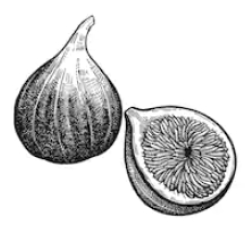
\includegraphics[width=1in,height=1.25in,clip,keepaspectratio]{fig1}}]{Michael Shell}
% Use $\backslash${\tt{begin\{IEEEbiography\}}} and then for the 1st argument use $\backslash${\tt{includegraphics}} to declare and link the author photo.
% Use the author name as the 3rd argument followed by the biography text.
% \end{IEEEbiography}

% \vspace{11pt}

% \bf{If you will not include a photo:}\vspace{-33pt}
% \begin{IEEEbiographynophoto}{John Doe}
% Use $\backslash${\tt{begin\{IEEEbiographynophoto\}}} and the author name as the argument followed by the biography text.
% \end{IEEEbiographynophoto}




\vfill

\end{document}


